\documentclass[../report.tex]{subfiles}
\begin{document}

\subsection{Discrete Services}

	The application was decided to be split in to discrete components with an all of the data processing  bundled together behind a single API exposed via HTTP with mostly JSON payloads (the observation data is transferred and stored in its original binary format).  The interface is a separate service that is mostly an HTML and JavaScript powered application that speaks to the API on the HTTP/JSON interface.  A third instance of the application runs to carry out long running or deferred tasks and is communicated with via Redis as a message queue.  Additionally data persistence services (see \cref{sec:data-persistence}) run separately.
	
\begin{figure}[h]
	\centering
	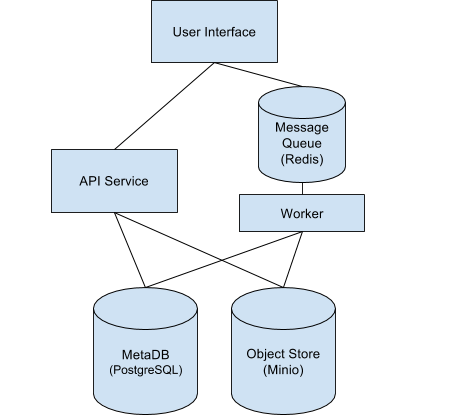
\includegraphics[width=.5\linewidth]{img/architecture}
	\caption{Application Architecture}
	\label{fig:architecture}
\end{figure}

\subsection{Data processing API}

	As previously mentioned, the data processing functions are bundled in to a single API process broken in to separate namespaces for the different parts.

	The \textit{observations} namespace used to manipulate observation files.  It supports a REST like interface for CRUD (Create, Read, Update and Delete) operations and RPCs (Remote Procedure Calls) for running event detection and retrieving results.
	
	The \textit{sax} namespace is exposed via a JSON based HTTP API.  Its purpose is to perform PAA and SAX operations on a given observation or event and return data for rendering visualisations as well as the produced string from the SAX calculation.
	
	The HTTP/JSON APIs were written using Flask-Restplus \citep{restplus}, a Python framework based on Flask that allows for request and response definition using Python Decorators around classes and methods.  The framework allows for dynamic generation of a swagger.json and provides a Swagger interface.  Swagger is a commonly used standard for defining APIs.  It also provides a user friendly HTML based interface for testing methods and calls during development and also doubles as API documentation.  An example of Swagger used on the Suffix Tree API is shown in \cref{fig:api}.
	
\begin{figure}[ht]
	\centering
	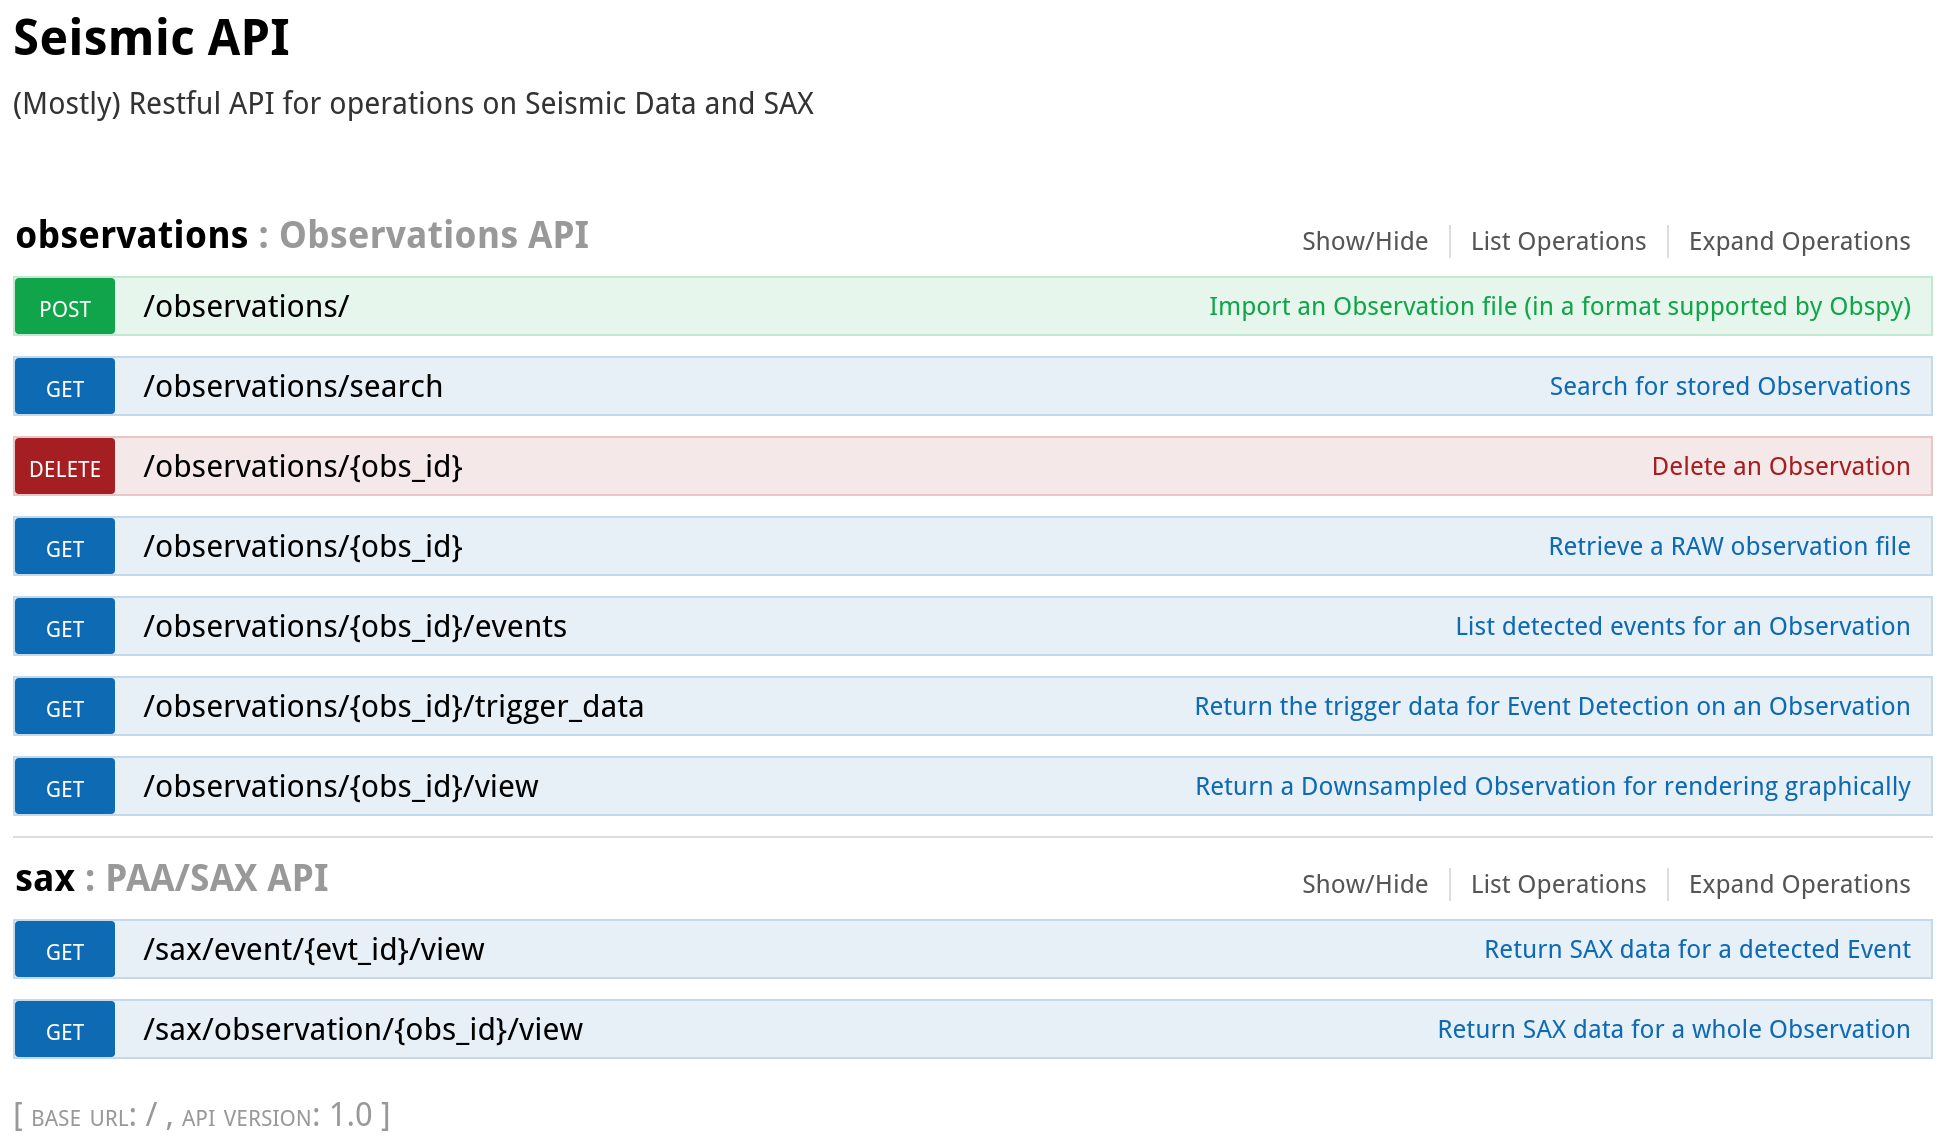
\includegraphics[width=1\linewidth]{img/api}
	\caption{Swagger interface for Data Processing API}
	\label{fig:api}
\end{figure}

\subsubsection{Observations API Namespace}
\subsubsection{SAX API Namespace}

\subsection{Data Persistence} \label{sec:data-persistence}
	For the persistence of Metadata about observations, detected events and Suffix Trees, PostgreSQL was selected.  PostgreSQL is a performant and mature open-source Relational Database Management System (RDBMS).  Being a fully featured RDBMS means it brings ACID guarantees for data resilience and transaction management.
	
	For the persistence of Binary objects (such as Raw Observation Files and Suffix Trees), Minio was selected.  Minio is an open-source object storage application written in Golang designed to emulate the abilities of Amazons Simple Storage Service (S3).  It allows for arbitrary binary objects to be stored and retrieved remotely from \textit{buckets} of grouped resources.  In each bucket, an object has a unique name that can also emulate a filesystem path (e.g. \textit{bucket}/somedir/somefile).
	
	A wrapper class was written around Minio that provides Get, Put and Delete operations.  This interface was intentionally left simple so that it could be replaced easily by another object or file store.
	
\subsection{User Interface}
	The user entry point to the application is served by the \textit{interface} service.  This provides a web based interface to the various backend components and rendering of graphs as well as acting as a reverse proxy to the various APIs behind the application.
	
	As mentioned previously, the interface to the application is web-based.  This serves two purposes; firstly it provides a unified experience across operating systems and secondly some of the processing can be memory and CPU intensive so is better suited for running on server hardware.  It also facilitates the potential sharing of data between users.
	
	The interface is served using Flask for Python.  Flask allows for dynamic request handling by converting URL paths directly in to function calls in Python.  It also supports HTML templating via Jinja2.  An module was written to act as a reverse proxy to expose various sections of the backend APIs to the browser.
	
	The view and control components of the interface were written in HTML (using Twitter's Bootstrap) and Javascript (using AngularJS, Charts.js and c3.js).  AngularJS allows for two way data binding between the Broswers DOM and elements such as form inputs and renders with minimal additional code.  It also provides a mechanism for sending requests to the APIs exposed by the aforementioned Proxy module.  Chart.js and c3.js are two open source Javascript charting libraries that utilise features included in HTML5 used in this case for rendering observation data.


\subsection{Deferred \& Batch Jobs} \label{sec:worker}
	For the running of deferred and batch jobs, Celery (another Python based project) was selected.  It uses a message queue for receiving and dispatching jobs.  Celery allows for the definition of jobs as functions which can then be imported by other processes (in this case, mostly the user interface).  The application uses Redis as the message queue. It also allows for the chaining together of tasks to ensure order (e.g. event detection before SAX analysis) and the passing of results on to the next function in a functional programming style.
	
\subsection{Suffix API}
	The Suffix API runs as a separate service as the majority of the code base is taken from previous work on suffix trees at Birkbeck \citep{bbk-suffix}.  This was done mainly to separate it from the original work on this project.  The only additions were an HTTP API written in the same style as the Data Processing API so that it could be interacted with.  The API operations are summarised in \cref{fig:suffix-api}.

\begin{figure}[ht]
	\centering
	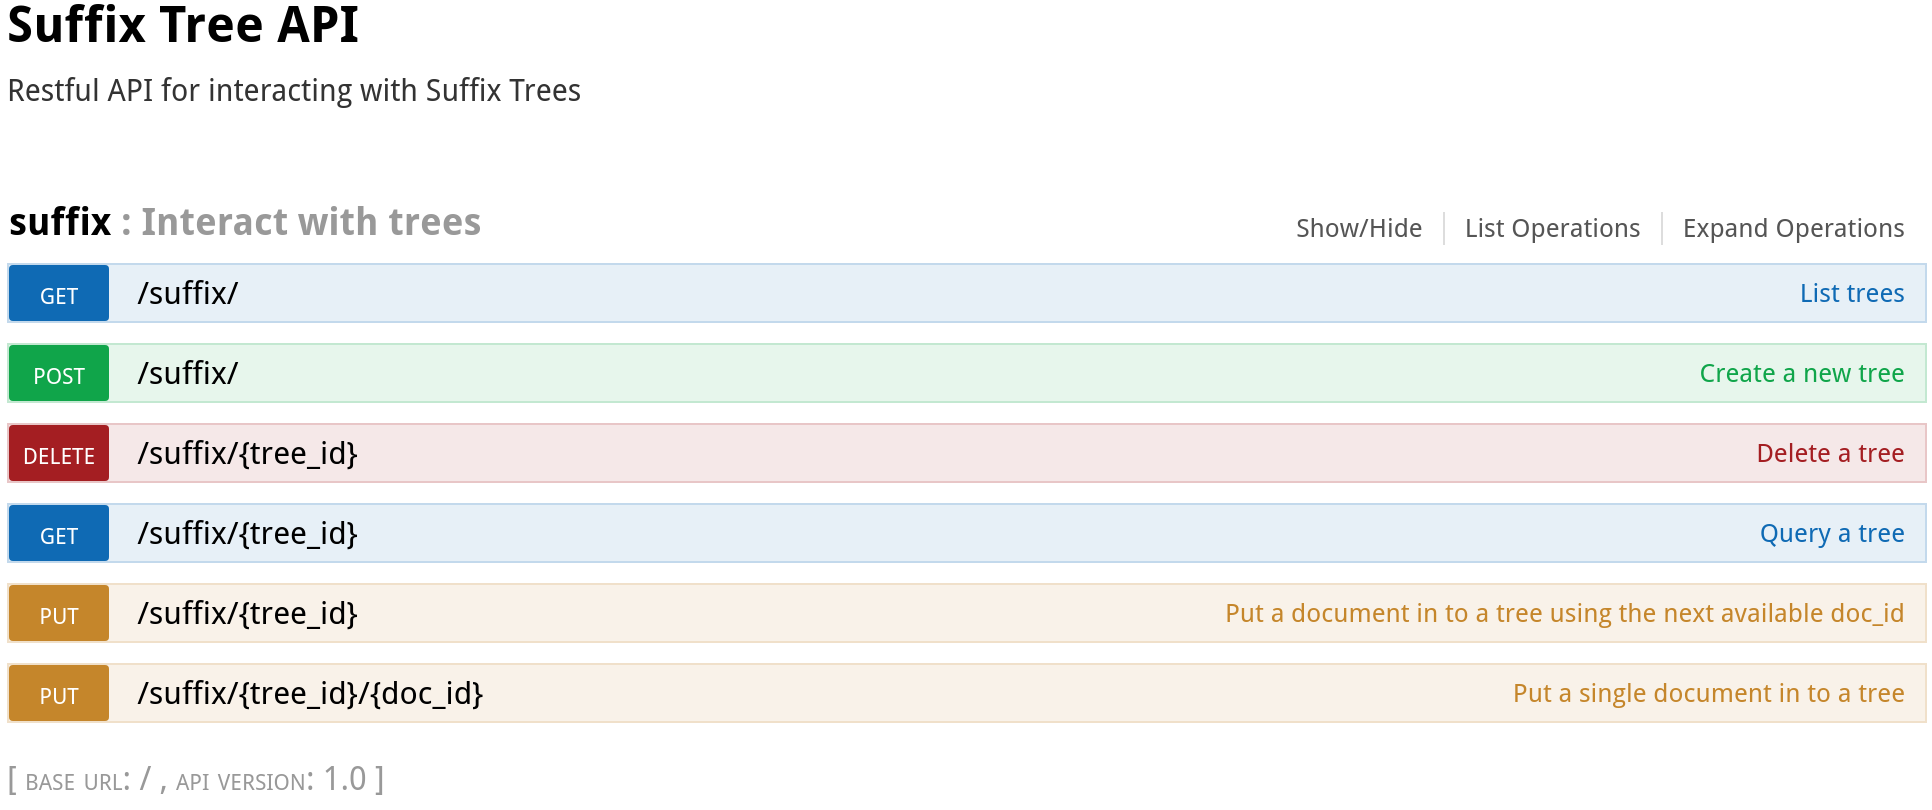
\includegraphics[width=1\linewidth]{img/suffix-api}
	\caption{Swagger interface for Suffix Tree API}
	\label{fig:suffix-api}
\end{figure}

%\begin{figure}[h]
%	\centering
%	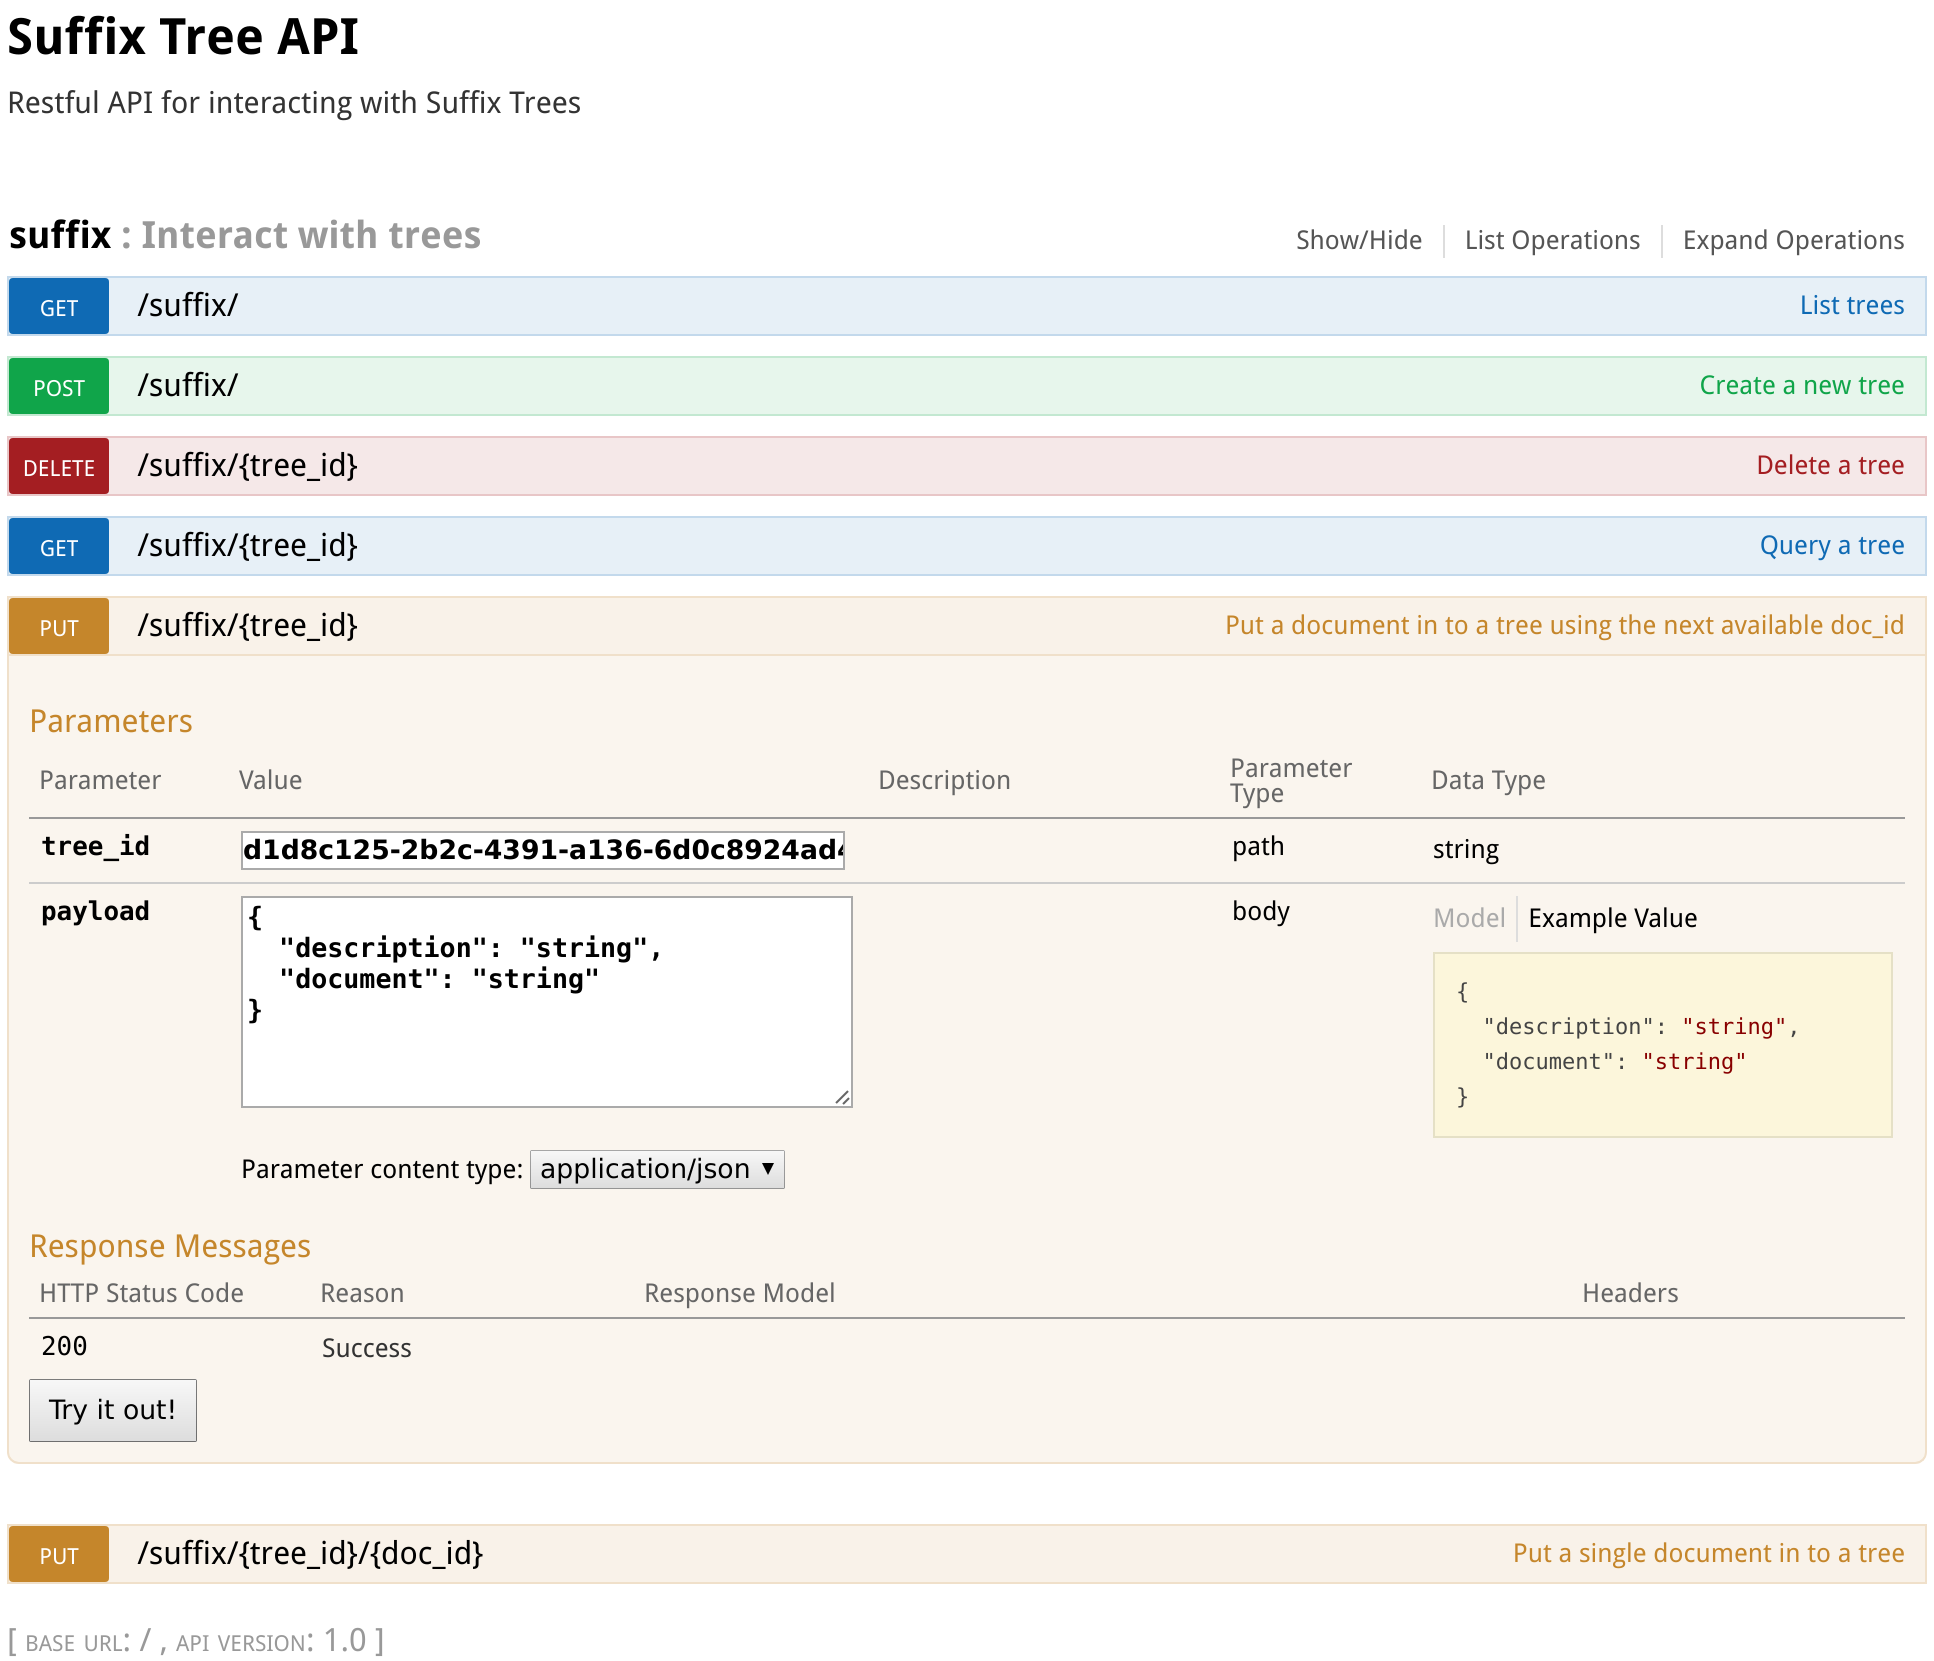
\includegraphics[width=1\linewidth]{img/swagger}
%	\caption{Swagger interface for Suffix Tree API}
%	\label{fig:swagger}
%\end{figure}
	
\end{document}